\chapter{}\label{chp:3}
We introduce a set $P_i$ for each job $i$, with $1 \leq i \leq n$, which contains the jobs that have to be finished before $i$ can start, and where $n$ is the total number of jobs. We let $s_i$ denote the time at which job $i$ started its execution. The time at which job $i$ finishes, $e_i$, can then be found as $e_i = s_i + i + 10$. To order the jobs, we need the starting time of some job $i$ to be later than the finishing times of all jobs in $P_i$. We get the constraint specified in Equation~\ref{order}.
\begin{equation}
    \label{order}
    \bigwedge^{n}_{i=1}\big(\bigwedge_{j\in P_i} s_i \geq (e_j)\big)
\end{equation}

Under these constraints, we want to minimize the total time it takes to execute all jobs. The total time is equal to the finishing time of the last finished job, and we get the following minimization objective:
\begin{equation}
    \textbf{Minimize: }\max_{1\leq i \leq n}(e_i)
\end{equation}

In the situation given by the assignment, we have the following sets $P$:
\begin{itemize}
    \item $P_3 = \{1,2\}$
    \item $P_6 = \{2,4\}$
    \item $P_7 = \{1,4,5\}$
    \item $P_8 = \{3,6\}$
    \item $P_9 = \{6,7\}$
    \item $P_{10} = \{8,9\}$
\end{itemize}
We use Z3 to find the results. To generate the SMT-LIB v2 file containing the constraints, we used a python script that can be found in \Cref{app:2_gen.py}. The resulting SMT-LIB v2 file can be found in \Cref{app:2_req.smt}. To interpret the results below, we created the script that can be found in \Cref{app:2_draw.py}. The resulting job scheduling of assignment (a) can be seen in Figure~\ref{fig:3a}.
\begin{figure}[H]
    \centering
    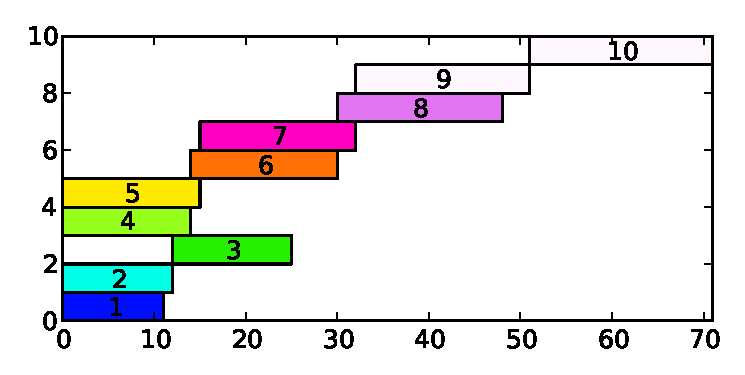
\includegraphics[width=\columnwidth]{3/a.out.pdf}
    \caption{A job scheduling for (a) where the total running time is minimized.}
    \label{fig:3a}
\end{figure}

To add the additional requirement of (b), we introduce another set $Q_i$ for every job $i$. Then, $Q_i$ contains the jobs $j$ for which $i$ is not allowed to start earlier than $j$. In other words, the starting time of $i$ can not be later than the starting time of $j$. This leads to the addition of the constraint specified in Equation~\ref{earlier}.
\begin{equation}
    \label{earlier}
    \bigwedge^{10}_{i=1}\big(\forall_{j\in Q_i} s_i \geq s_i \geq s_j \big)
\end{equation}

The given requirement and situation given by the assignment results in the following set $Q$:
\begin{itemize}
    \item $Q_7 = \{8\}$
\end{itemize}
The results can be seen in Figure~\ref{fig:3b}.
\begin{figure}[H]
    \centering
    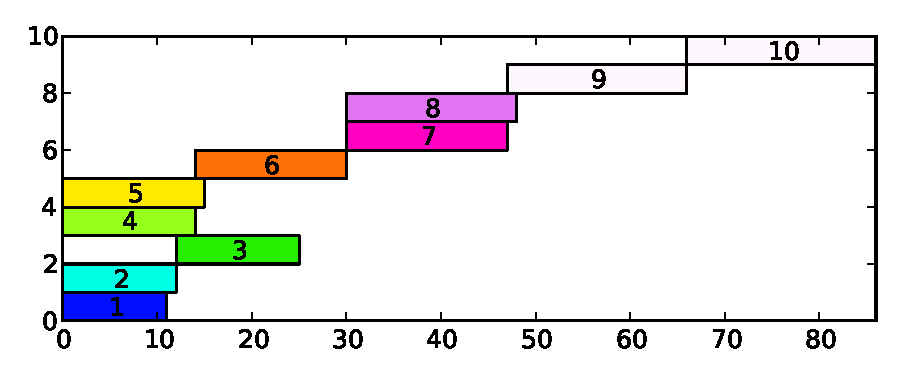
\includegraphics[width=\columnwidth]{3/b.out.pdf}
    \caption{A job scheduling for (b) where the total running time is minimized.}
    \label{fig:3b}
\end{figure}

For (c), we again introduce an additional set $R_i$ for every job $i$. Now, $R_i$ contains the jobs $j$ which $i$ is not allowed to run in parallel with. This means that for each $j \in Q_i$, the starting time of $s_i$ can not be in the range $(s_j - (i + 10), s_j + j + 10)$. Note that when we for instance have $R_6 = \{4\}$, it is not required to also have $6 \in R_4$, as $R_6$ already forces mutual exclusion between jobs 6 and 4. The resulting constraint is specified in Equation~\ref{mutex}.
\begin{equation}
    \label{mutex}
    \bigwedge^{10}_{i=1}\bigg(\forall_{j \in R_i}\big((s_i \geq s_j + j + 10) \vee (s_i + i + 10 \leq s_j)\big)\bigg)
\end{equation}
The results for (c) can be seen in Figure~\ref{fig:3c}.
\begin{figure}[H]
    \centering
    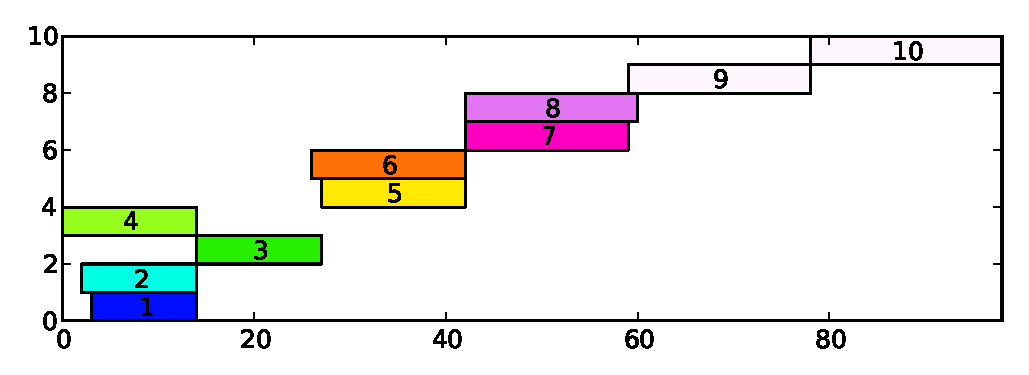
\includegraphics[width=\columnwidth]{3/c.out.pdf}
    \caption{A job scheduling for (c) where the total running time is minimized.}
    \label{fig:3c}
\end{figure}
